\documentclass[journal,12pt,twocolumn]{IEEEtran}

\usepackage{setspace}
\usepackage{gensymb}
\singlespacing
\usepackage[cmex10]{amsmath}

\usepackage{amsthm}

\usepackage{mathrsfs}
\usepackage{txfonts}
\usepackage{stfloats}
\usepackage{bm}
\usepackage{cite}
\usepackage{cases}
\usepackage{subfig}

\usepackage{longtable}
\usepackage{multirow}

\usepackage{enumitem}
\usepackage{mathtools}
\usepackage{steinmetz}
\usepackage{tikz}
\usepackage{circuitikz}
\usepackage{verbatim}
\usepackage{tfrupee}
\usepackage[breaklinks=true]{hyperref}
\usepackage{graphicx}
\usepackage{tkz-euclide}

\usetikzlibrary{calc,math}
\usepackage{listings}
    \usepackage{color}                                            %%
    \usepackage{array}                                            %%
    \usepackage{longtable}                                        %%
    \usepackage{calc}                                             %%
    \usepackage{multirow}                                         %%
    \usepackage{hhline}                                           %%
    \usepackage{ifthen}                                           %%
    \usepackage{lscape}     
\usepackage{multicol}
\usepackage{chngcntr}

\DeclareMathOperator*{\Res}{Res}
\newtheorem{theorem}{Theorem}[section]
\newtheorem{corollary}{Corollary}[theorem]
\newtheorem{lemma}[theorem]{Lemma}
\newtheorem{definition}{Definition}[section]
\renewcommand\thesection{\arabic{section}}
\renewcommand\thesubsection{\thesection.\arabic{subsection}}
\renewcommand\thesubsubsection{\thesubsection.\arabic{subsubsection}}

\renewcommand\thesectiondis{\arabic{section}}
\renewcommand\thesubsectiondis{\thesectiondis.\arabic{subsection}}
\renewcommand\thesubsubsectiondis{\thesubsectiondis.\arabic{subsubsection}}


\hyphenation{op-tical net-works semi-conduc-tor}
\def\inputGnumericTable{}                                 %%

\lstset{
%language=C,
frame=single, 
breaklines=true,
columns=fullflexible
}
\begin{document}

\newcommand{\BEQA}{\begin{eqnarray}}
\newcommand{\EEQA}{\end{eqnarray}}
\newcommand{\define}{\stackrel{\triangle}{=}}
\bibliographystyle{IEEEtran}
\raggedbottom
\setlength{\parindent}{0pt}
\providecommand{\mbf}{\mathbf}
\providecommand{\pr}[1]{\ensuremath{\Pr\left(#1\right)}}
\providecommand{\qfunc}[1]{\ensuremath{Q\left(#1\right)}}
\providecommand{\sbrak}[1]{\ensuremath{{}\left[#1\right]}}
\providecommand{\lsbrak}[1]{\ensuremath{{}\left[#1\right.}}
\providecommand{\rsbrak}[1]{\ensuremath{{}\left.#1\right]}}
\providecommand{\brak}[1]{\ensuremath{\left(#1\right)}}
\providecommand{\lbrak}[1]{\ensuremath{\left(#1\right.}}
\providecommand{\rbrak}[1]{\ensuremath{\left.#1\right)}}
\providecommand{\cbrak}[1]{\ensuremath{\left\{#1\right\}}}
\providecommand{\lcbrak}[1]{\ensuremath{\left\{#1\right.}}
\providecommand{\rcbrak}[1]{\ensuremath{\left.#1\right\}}}
\theoremstyle{remark}
\newtheorem{rem}{Remark}
\newtheorem*{remark}{Remark}
\newcommand{\sgn}{\mathop{\mathrm{sgn}}}
\providecommand{\abs}[1]{\vert#1\vert}
\providecommand{\res}[1]{\Res\displaylimits_{#1}} 
\providecommand{\norm}[1]{\lVert#1\rVert}
%\providecommand{\norm}[1]{\lVert#1\rVert}
\providecommand{\mtx}[1]{\mathbf{#1}}
\providecommand{\mean}[1]{E[ #1 ]}
\providecommand{\fourier}{\overset{\mathcal{F}}{ \rightleftharpoons}}
%\providecommand{\hilbert}{\overset{\mathcal{H}}{ \rightleftharpoons}}
\providecommand{\system}{\overset{\mathcal{H}}{ \longleftrightarrow}}
	%\newcommand{\solution}[2]{\textbf{Solution:}{#1}}
\newcommand{\solution}{\noindent \textbf{Solution: }}
\newcommand{\cosec}{\,\text{cosec}\,}
\providecommand{\dec}[2]{\ensuremath{\overset{#1}{\underset{#2}{\gtrless}}}}
\newcommand{\myvec}[1]{\ensuremath{\begin{pmatrix}#1\end{pmatrix}}}
\newcommand{\mydet}[1]{\ensuremath{\begin{vmatrix}#1\end{vmatrix}}}
\numberwithin{equation}{subsection}
\makeatletter
\@addtoreset{figure}{problem}
\makeatother
\let\StandardTheFigure\thefigure
\let\vec\mathbf
\renewcommand{\thefigure}{\theproblem}
\def\putbox#1#2#3{\makebox[0in][l]{\makebox[#1][l]{}\raisebox{\baselineskip}[0in][0in]{\raisebox{#2}[0in][0in]{#3}}}}
     \def\rightbox#1{\makebox[0in][r]{#1}}
     \def\centbox#1{\makebox[0in]{#1}}
     \def\topbox#1{\raisebox{-\baselineskip}[0in][0in]{#1}}
     \def\midbox#1{\raisebox{-0.5\baselineskip}[0in][0in]{#1}}
\vspace{3cm}
\title{Quiz 1}
\author{Yashas Tadikamalla - AI20BTECH11027}
\maketitle
\newpage
\bigskip
\renewcommand{\thefigure}{\theenumi}
\renewcommand{\thetable}{\theenumi}
Download all python codes from 
\begin{lstlisting}
https://github.com/YashasTadikamalla/EE3900/blob/main/Quiz1/codes
\end{lstlisting}
%
and latex-tikz codes from 
%
\begin{lstlisting}
https://github.com/YashasTadikamalla/EE3900/blob/main/Quiz1/Quiz1.tex
\end{lstlisting}
\section{Problem (2.29 (c,d))}
A discrete-time signal $x[n]$ is shown in figure below
\begin{figure}[!h]
 \centering
 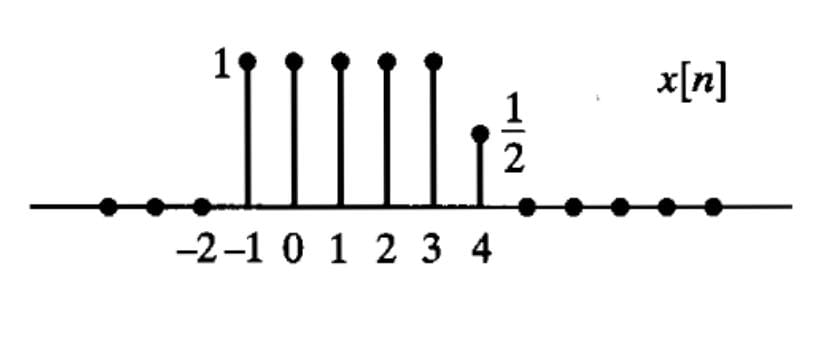
\includegraphics[width=\columnwidth]{Quiz1.jpeg}
 \caption{$x[n]$}
 \label{plot}
\end{figure}


Sketch and label carefully, each of the following signals:
\begin{enumerate}
    \item $x[2n]$
    \item $x[n]u[2-n]$
\end{enumerate}
\section{Solution}
Given, $\forall n \in \mathbb{Z}$
\begin{align}
    x[n]=\begin{cases}
	0, & n \leq -2 \\~\\[-1em]
	1, & -1 \leq n \leq 3 \\~\\[-1em]
	\dfrac{1}{2}, & n=4 \\~\\[-1em]
	0, & n \geq 5 
	\end{cases}
	\label{eq:x}
\end{align}
Also, $\forall n \in \mathbb{Z}$
\begin{align}
    u[n]=\begin{cases}
	0, & n \leq -1 \\~\\[-1em]
	1, & n \geq 0 
	\end{cases}
	\label{eq:u}
\end{align}
\begin{enumerate}
\item To find: $x[2n]$. From \eqref{eq:x},
\begin{align}
    x[n]&=0, n\leq -2 \text{ and } n\geq 5\\
    \Rightarrow x[2n]&=0, 2n\leq -2 \text{ and } 2n\geq 5\\
    \Rightarrow y[n]&=0, n\leq -1 \text{ and } n\geq 3 \brak{\because n \in \mathbb{Z}}
\end{align}
Now, we just need to check for values of $x[2n]$ for $n=0,1,2$.
\begin{align}
    x[2*0]&=x[0]=1\\
    x[2*1]&=x[2]=1\\
    x[2*2]&=x[4]=\dfrac{1}{2}
\end{align}
Hence, $\forall n \in \mathbb{Z}$
\begin{align}
    x[2n]=\begin{cases}
	0, & n \leq -1 \\~\\[-1em]
	1, & 0 \leq n \leq 1 \\~\\[-1em]
	\dfrac{1}{2}, & n=2 \\~\\[-1em]
	0, & n \geq 3
	\end{cases}
	\label{eq:y}
\end{align}
\begin{figure}[!h]
 \centering
 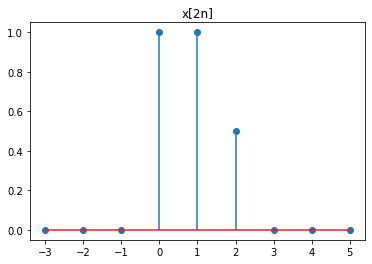
\includegraphics[width=\columnwidth]{Quiz1(1).png}
 \caption{Plot of $x[2n]$}
 \label{plot}
\end{figure}
\item To find: $x[n]u[2-n]$. From \eqref{eq:u}
\begin{align}
    u[2-n]=\begin{cases}
	0, & n \geq 3 \\~\\[-1em]
	1, & n \leq 2
	\end{cases}
	\label{eq:u2-n}
\end{align}
From \eqref{eq:x},\eqref{eq:u2-n}
\begin{align}
    x[n]u[2-n]=0, n\leq -2 \text{ and } n\geq 3
\end{align}
Now, we just need to check for values of $x[n]u[2-n]$ for $n=-1,0,1,2$.
\begin{align}
    x[-1]u[2-(-1)]&=x[-1]u[3]=1\\
    x[0]u[2-0]&=x[0]u[2]=1\\
    x[1]u[2-1]&=x[2]u[1]=1\\
    x[2]u[2-2]&=x[4]u[0]=1
\end{align}
Hence, $\forall n \in \mathbb{Z}$
\begin{align}
    x[n]u[2-n]=\begin{cases}
	0, & n \leq -2 \\~\\[-1em]
	1, & -1 \leq n \leq 2 \\~\\[-1em]
	0, & n \geq 3
	\end{cases}
	\label{eq:z}
\end{align}
\begin{figure}[!h]
 \centering
 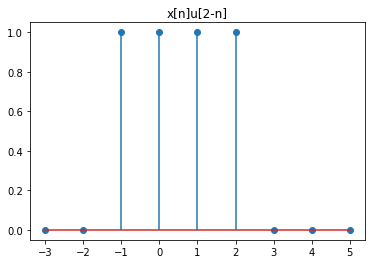
\includegraphics[width=\columnwidth]{Quiz1(2).png}
 \caption{Plot of $x[n]u[2-n]$}
 \label{plot}
\end{figure}
\end{enumerate}
\end{document}


